\begin{figure*}[h]
\centering
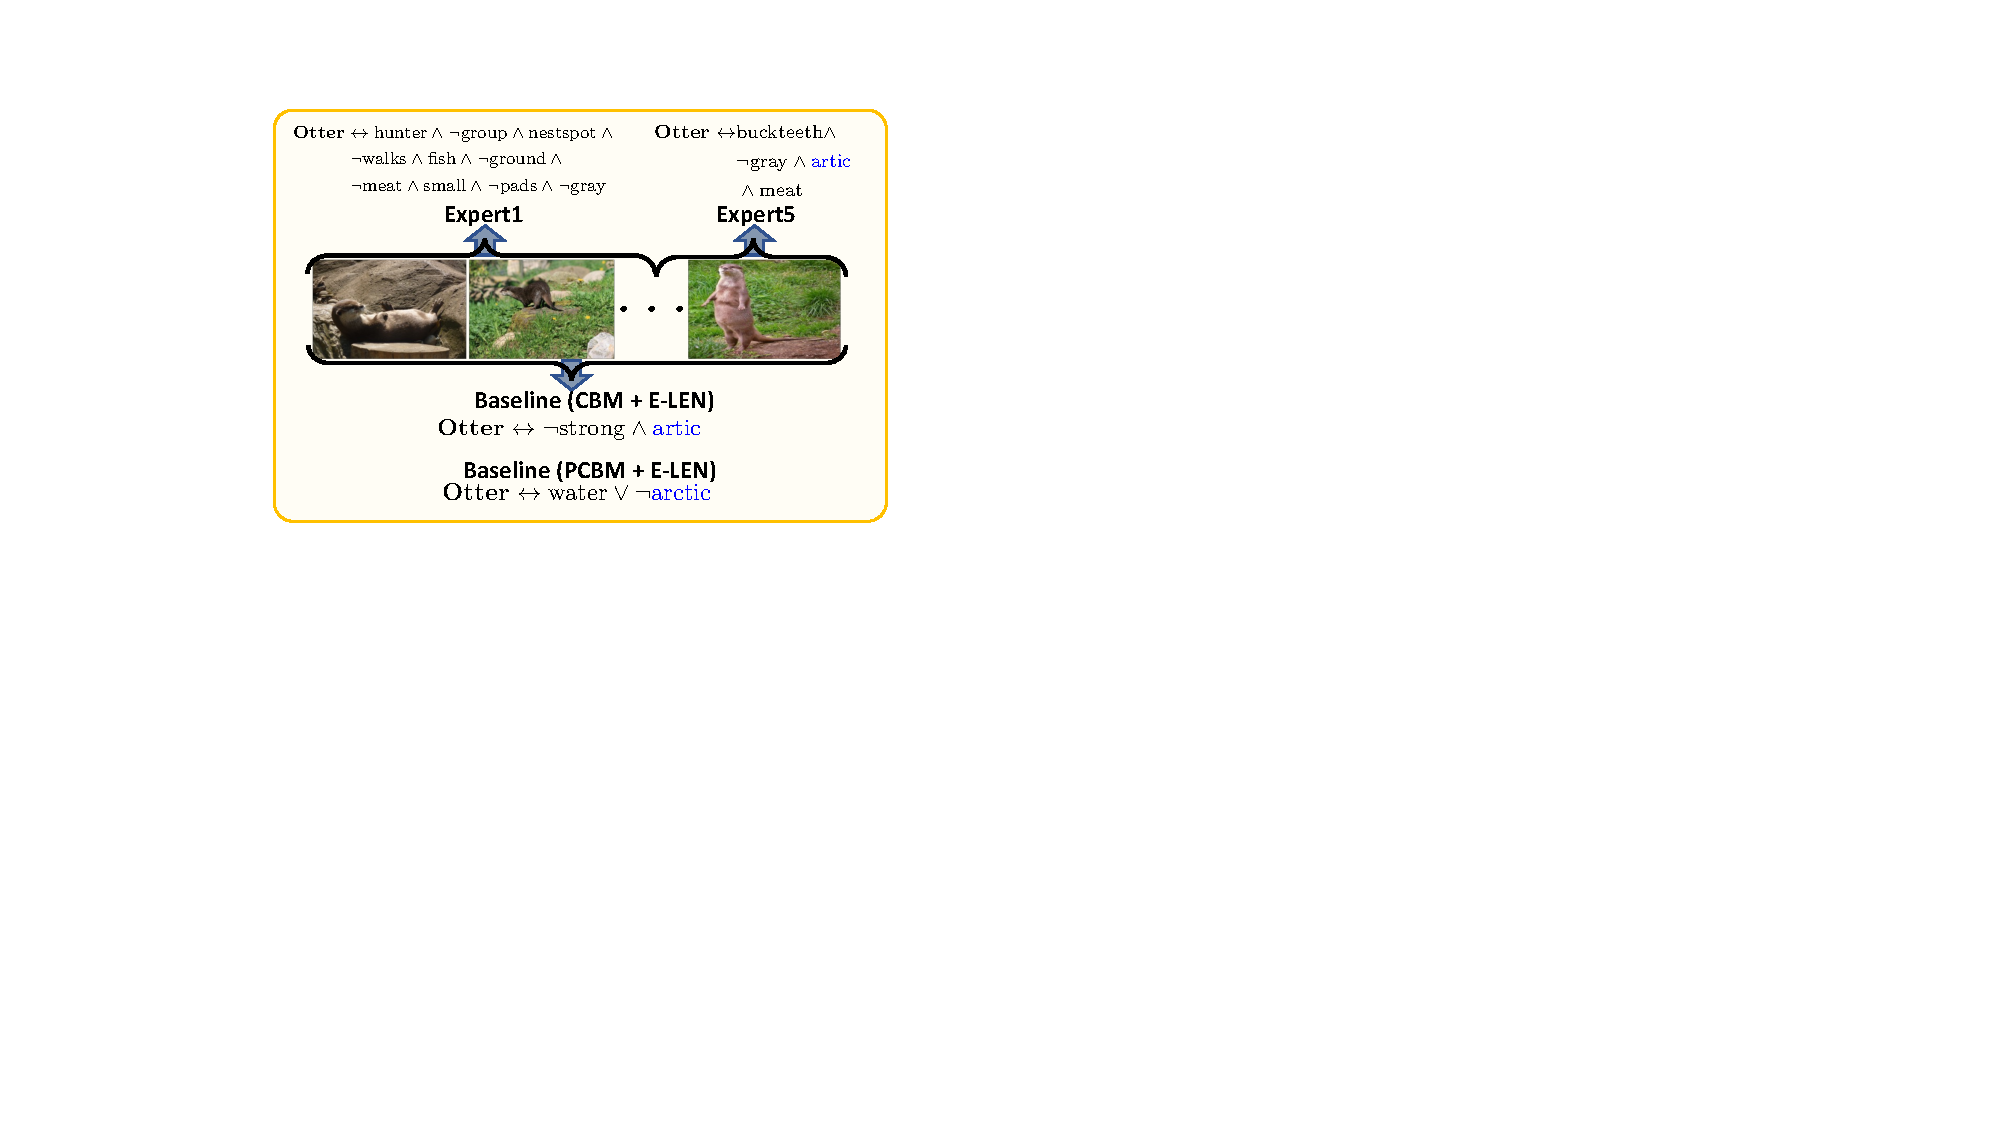
\includegraphics[width=\columnwidth]{figures/Supp/Local_awa2_otter.pdf}
\vspace{-10pt}
\caption{Flexibility of FOL explanations by VIT-derived MoIE  MoIE and the CBM + E-LEN and PCBM + E-LEN baselines for Awa2 dataset to classify ``Otter'' at inference. Both the baseline's FOL constitutes identical concepts to distinguish all the samples. However, expert1 classifies ``Otter'' with \textit{hunter}, \textit{group} \etc as the identifying concept for the instances covered by it. Similarly expert5 classifies ``Otter'' using \textit{buckteeth}, \textit{gray} \etc. Note that, \textit{meat} and \textit{gray}  are shared between the two experts. We highlight the shared concepts (\textit{artic}) between the experts and the baselines as blue.}
\label{fig:local_awa2_otter}
\vspace{-2.5pt}
\end{figure*}

\begin{figure*}[h]
\centering
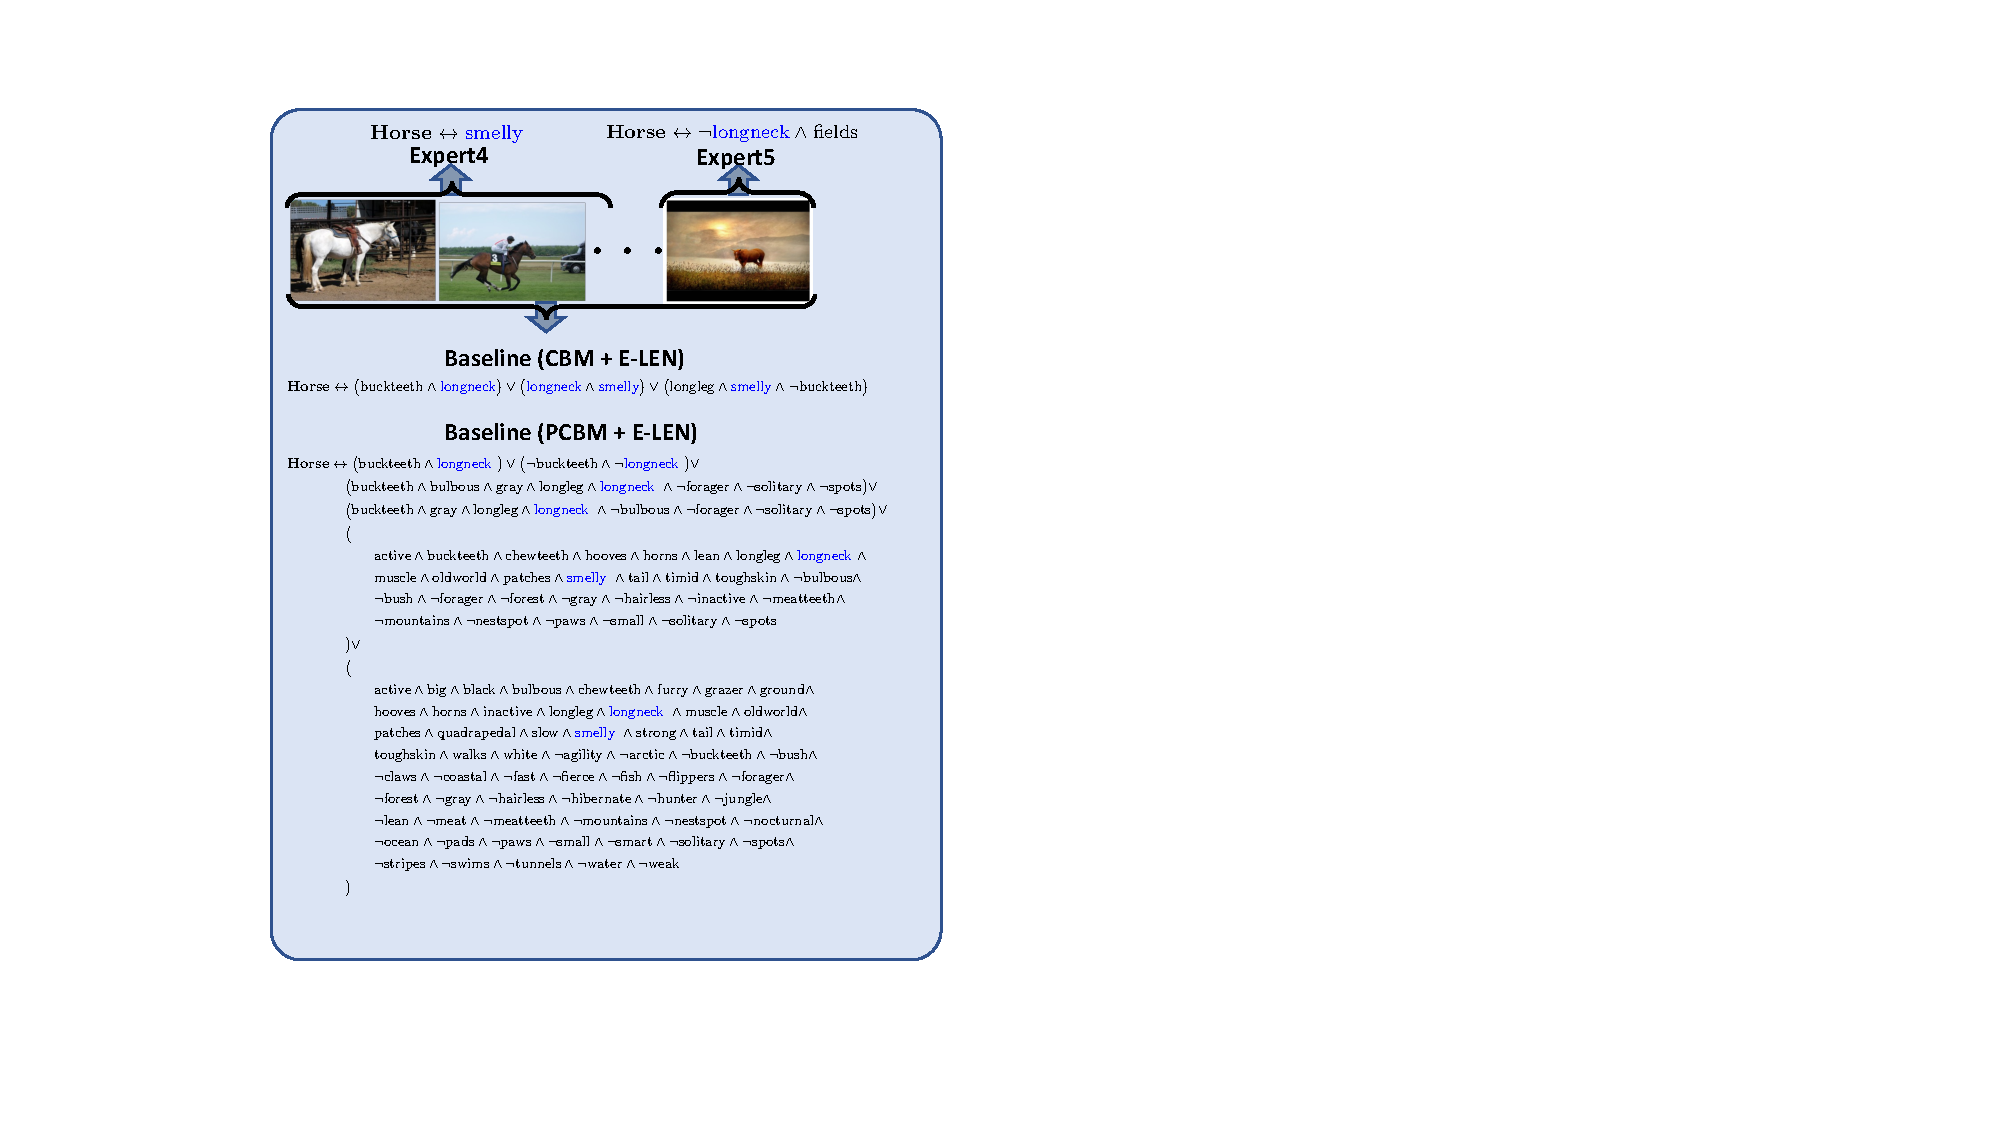
\includegraphics[width=\columnwidth]{figures/Supp/Local_awa2_horse.pdf}
\vspace{-10pt}
\caption{Flexibility of FOL explanations by VIT-derived MoIE  MoIE and the CBM + E-LEN and PCBM + E-LEN baselines for Awa2 dataset to classify ``Horse'' at inference. Both the baseline's FOL constitutes identical concepts to distinguish all the samples. However, expert4 classifies ``Horse'' with \textit{smelly} as the identifying concept for the instances covered by it. Similarly, expert5 classifies the same ``Horse'' using \textit{longneck} and \textit{fields}. We highlight the shared concepts between the experts and the baselines as blue.}
\label{fig:local_awa2_horse}
\vspace{-2.5pt}
\end{figure*}

\cref{fig:local_awa2_otter} and~\ref{fig:local_awa2_horse} demonstrate the flexibility of FOL explanations by VIT-derived MoIE compared to the different baselines for the Awa2 dataset qualitatively.